\begin{figure}[t!]
\begin{tabular}{@{}c@{}c@{}}
\begin{subfigure}[b]{0.5\textwidth}
\begin{center}
{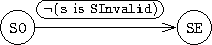
\includegraphics[scale=1.4]{chapters/figures/figIsEmptySpecCFG.pdf}}
\end{center}
\vspace{20px}
\caption{\label{fig:isemptyspeccfg}CFG of \SpecL{} procedure}
\end{subfigure}%
&
\begin{subfigure}[b]{0.5\textwidth}
\begin{center}
{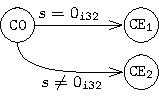
\includegraphics[scale=1.4]{chapters/figures/figIsEmptyCCFG.pdf}}
\end{center}
\caption{\label{fig:isemptyccfg}CFG of C procedure}
\end{subfigure}%
\\
\end{tabular}
\caption{\label{fig:isemptyspecandccfg}CFG representation of \SpecL{} and C IRs in \cref{fig:isemptyspecir,fig:isemptycir} for the {\tt is\_empty} procedures in \cref{fig:isemptyspec,fig:isemptyc} respectively.}
% \end{figure}
